%%%%%%%%%%%%%%%%%%%%%%%%%%%%%%%%%%%%%%%%%%%%%%%%%%%%%%%%%%%%%%%%%%%%%%%%
% Beamer Presentation - LaTeX - Template Version 1.0 (10/11/12)
% This template has been downloaded from: http://www.LaTeXTemplates.com
% License: % CC BY-NC-SA 3.0 (http://creativecommons.org/)
% Modified by Rahmat M. Samik-Ibrahim

% REV343 Wed 08 Sep 2021 21:50:50 WIB
% REV339 Sat 04 Sep 2021 12:50:36 WIB
% REV328 Sat 14 Aug 2021 13:11:51 WIB
% REV319 Mon 19 Jul 2021 23:57:40 WIB
% REV314 Fri 09 Jul 2021 05:29:31 WIB
% STARTX Wed Sep 14 10:45:19 WIB 2016
%%%%%%%%%%%%%%%%%%%%%%%%%%%%%%%%%%%%%%%%%%%%%%%%%%%%%%%%%%%%%%%%%%%%%%%%%

% PACKAGES AND THEMES 
\documentclass[xcolor=table, notheorems, hyperref={pdfpagelabels=false}]{beamer}
%%%%%%%%%%%%%%%%%%%%%%%%%%%%%%%%%%%%%%%%%%%%%%%%%%%%%%%%%%%%%%%%%%%%%%%%
% Beamer Presentation - LaTeX - Template Version 1.0 (10/11/12)
% This template has been downloaded from: http://www.LaTeXTemplates.com
% License: % CC BY-NC-SA 3.0 (http://creativecommons.org/)
% Modified by Rahmat M. Samik-Ibrahim
% REV316 Wed 14 Jul 2021 13:42:41 WIB
% REV217 Tue Feb  4 15:10:30 WIB 2020
% REV198 Wed Mar 13 16:39:02 WIB 2019
% REV006 Mon Jan 22 19:10:41 WIB 2018
% REV005 Mon Oct  2 14:45:07 WIB 2017
% START  Thu Aug 25 14:15:19 WIB 2016
%%%%%%%%%%%%%%%%%%%%%%%%%%%%%%%%%%%%%%%%%%%%%%%%%%%%%%%%%%%%%%%%%%%%%%%%%

%% ZCZC NNNN
\newtheorem{example}{Example}

%%%%%%%%%%%%%%%%%%%%%%%%%%%%%%%%%%%%%%%%%%%%%%%%%%%%%%%%%%%%%%%%%%%%%%%%%

\let\Tiny=\tiny
\mode<presentation> {
% The Beamer class comes with a number of default slide themes
% which change the colors and layouts of slides. Below this is a list
% of all the themes, uncomment each in turn to see what they look like.
%\usetheme{Boadilla}
\usetheme{Madrid}
% ZCZC %%%%%%%%%%%%%%%%%%%%%%%%%%%%%%%%%%%%%%%%%%%%%%%%%%%%%%%%%%%%%%%%%%
% \usetheme{default} \usetheme{AnnArbor} \usetheme{Antibes} \usetheme{Bergen}
% \usetheme{Berkeley} \usetheme{Berlin} \usetheme{CambridgeUS} 
% \usetheme{Copenhagen} \usetheme{Darmstadt} \usetheme{Dresden}
% \usetheme{Frankfurt} \usetheme{Goettingen} \usetheme{Hannover}
% \usetheme{Ilmenau} \usetheme{JuanLesPins} \usetheme{Luebeck}
% \usetheme{Malmoe} \usetheme{Marburg} \usetheme{Montpellier}
% \usetheme{PaloAlto} \usetheme{Pittsburgh} \usetheme{Rochester}
% \usetheme{Singapore} \usetheme{Szeged} \usetheme{Warsaw}
% NNNN %%%%%%%%%%%%%%%%%%%%%%%%%%%%%%%%%%%%%%%%%%%%%%%%%%%%%%%%%%%%%%%%%%
% As well as themes, the Beamer class has a number of color themes
% for any slide theme. Uncomment each of these in turn to see how it
% changes the colors of your current slide theme.
%\usecolortheme{orchid}
%\usecolortheme{rose}
%\usecolortheme{seagull}
%\usecolortheme{seahorse}
\usecolortheme{whale}
% ZCZC %%%%%%%%%%%%%%%%%%%%%%%%%%%%%%%%%%%%%%%%%%%%%%%%%%%%%%%%%%%%%%%%%%
%\usecolortheme{albatross} \usecolortheme{beaver} \usecolortheme{beetle}
%\usecolortheme{crane} \usecolortheme{dolphin} \usecolortheme{dove}
%\usecolortheme{fly} \usecolortheme{lily} \usecolortheme{wolverine}
% NNNN %%%%%%%%%%%%%%%%%%%%%%%%%%%%%%%%%%%%%%%%%%%%%%%%%%%%%%%%%%%%%%%%%%
% To remove the footer line in all slides uncomment this line
%\setbeamertemplate{footline} 
% To replace the footer line in all slides uncomment this line
%\setbeamertemplate{footline}[page number] 
% To remove the navigation symbols from the bottom uncomment this line
\setbeamertemplate{navigation symbols}{} 
}

\usepackage{array}       % ZCZC
\usepackage{amssymb}     % ZCZC
\usepackage{bold-extra}  % ZCZC
\usepackage{booktabs}    % Allows \toprule, \midrule and \bottomrule in tables
\usepackage{caption}
\usepackage[T1]{fontenc} % ZCZC << >>
\usepackage{graphicx}    % Allows including images
\usepackage{listings}    % listing
\usepackage{lmodern}     % ZCZC
\usepackage{perpage}     % reset footnote per page
\usepackage{geometry}    % ZCZC
\usepackage{adjustbox}   % ZCZC
\usepackage{multirow}    % ZCZC

% \definecolor{links}{HTML}{2A1B81}
\definecolor{links}{HTML}{0011FF}
\hypersetup{colorlinks,linkcolor=,urlcolor=links}

% \usepackage{xcolor}
% \usepackage[colorlinks = true,
%             linkcolor = blue,
%             urlcolor  = blue,
%             citecolor = blue,
%             anchorcolor = blue]{hyperref}

\captionsetup[table]{name=Tabel}
\makeatletter
\def\input@path{{src/}}
\makeatother
\graphicspath{{src/}}      % src directory
\MakePerPage{footnote}     % reset page

% NNNN %%%%%%%%%%%%%%%%%%%%%%%%%%%%%%%%%%%%%%%%%%%%%%%%%%%%%%%%%%%%%%%%%%

%% % XXXXXXXXXXXXXXXXXXXXXXXXXXXXXXXXXXXXXXXXXXXXXXXXXXXXXXXXXXXXXXXXXXXXXXXXXX
%% % The short title appears at the bottom of every slide, 
%% % the full title is only on the title page
%% \title[Judul Pendek]{Judul Panjang dan Lengkap} 
%% \author{Cecak bin Kadal}
%% \institute[UILA]
%% {
%% University of Indonesia at Lenteng Agung \\ 
%% \medskip
%% \textit{cecak@binKadal.com}
%% }
%% \date{REV00 24-Aug-2016}
%% % \date{\today}
%% 

%% % XXXXXXXXXXXXXXXXXXXXXXXXXXXXXXXXXXXXXXXXXXXXXXXXXXXXXXXXXXXXXXXXXXXXXXXXXX
%% \begin{document}
%% \section{Judul}
%% \begin{frame}
%% \titlepage
%% \end{frame}
%% 
%% % XXXXXXXXXXXXXXXXXXXXXXXXXXXXXXXXXXXXXXXXXXXXXXXXXXXXXXXXXXXXXXXXXXXXXXXXXX
%% \section{Agenda}
%% \begin{frame}
%% \frametitle{Agenda}
%% % Throughout your presentation, if you choose to use \section{} and 
%% % \subsection{} commands, these will automatically be printed on 
%% % this slide as an overview of your presentation
%% \tableofcontents 
%% \end{frame}
%% 
%% % XXXXXXXXXXXXXXXXXXXXXXXXXXXXXXXXXXXXXXXXXXXXXXXXXXXXXXXXXXXXXXXXXXXXXXXXXX
%% \section{UUD dan Pancasila}
%% \subsection{UUD}
%% \begin{frame}
%% \frametitle{Pembukaan}
%% Bahwa sesungguhnya kemerdekaan itu ialah hak segala bangsa dan oleh 
%% sebab itu, maka penjajahan diatas dunia harus dihapuskan karena 
%% tidak sesuai dengan perikemanusiaan dan perikeadilan.
%% \\~\\
%% Atas berkat rahmat Allah Yang Maha Kuasa dan dengan didorongkan oleh 
%% keinginan luhur, supaya berkehidupan kebangsaan yang bebas, maka 
%% rakyat Indonesia menyatakan dengan ini kemerdekaannya.
%% \end{frame}
%% 
%% % XXXXXXXXXXXXXXXXXXXXXXXXXXXXXXXXXXXXXXXXXXXXXXXXXXXXXXXXXXXXXXXXXXXXXXXXXX
%% \begin{frame}
%% \frametitle{Alenia Ketiga}
%% Kemudian daripada itu untuk membentuk suatu pemerintah negara Indonesia 
%% yang melindungi segenap bangsa Indonesia dan seluruh tumpah darah Indonesia 
%% dan untuk memajukan kesejahteraan umum, mencerdaskan kehidupan bangsa, dan 
%% ikut melaksanakan ketertiban dunia yang berdasarkan kemerdekaan, perdamaian 
%% abadi dan keadilan sosial, maka disusunlah kemerdekaan kebangsaan Indonesia 
%% itu dalam suatu Undang-Undang Dasar negara Indonesia, yang terbentuk dalam 
%% suatu susunan negara Republik Indonesia yang berkedaulatan rakyat dengan 
%% berdasar kepada:
%% \begin{itemize}
%% \item Ketuhanan Yang Maha Esa,
%% \item kemanusiaan yang adil dan beradab,
%% \item persatuan Indonesia,
%% \item dan kerakyatan yang dipimpin oleh hikmat kebijaksanaan 
%%       dalam permusyawaratan/ perwakilan,
%% \item serta dengan mewujudkan suatu keadilan sosial bagi seluruh rakyat 
%%       Indonesia.
%% \end{itemize}
%% \end{frame}
%% 
%% % XXXXXXXXXXXXXXXXXXXXXXXXXXXXXXXXXXXXXXXXXXXXXXXXXXXXXXXXXXXXXXXXXXXXXXXXXX
%% \subsection{Pancasila}
%% \begin{frame}
%% \frametitle{Tujuh Kunci Pokok}
%% \begin{block}{Pertama - Kedua - Ketiga}
%% Indonesia ialah negara berdasarkan hukum.
%% Sistem konstitusional.
%% Kekuasaan negara tertinggi di tangan MPR.
%% \end{block}
%% 
%% \begin{block}{Keempat - Kelima}
%% Presiden adalah penyelenggara pemerintahan tertinggi di bawah MPR.
%% Adanya pengawasan DPR.
%% \end{block}
%% 
%% \begin{block}{Keenam}
%% Menteri negara adalah pembantu presiden dan tidak bertanggung jawab 
%% kepada DPR.
%% \end{block}
%% 
%% \begin{block}{Ketujuh}
%% Kekuasaan kepala negara tidak tak tebatas.
%% \end{block}
%% 
%% \end{frame}
%% 
%% % XXXXXXXXXXXXXXXXXXXXXXXXXXXXXXXXXXXXXXXXXXXXXXXXXXXXXXXXXXXXXXXXXXXXXXXXXX
%% \section{Rupa-rupa}
%% \subsection{Kolom}
%% \begin{frame}
%% \frametitle{Kolom}
%% % The "c" option specifies centered vertical alignment 
%% % while the "t" option is used for top vertical alignment
%% \begin{columns}[c] 
%% % Left column and width
%% \column{.45\textwidth} 
%% \textbf{Heading}
%% \begin{enumerate}
%% \item Satu-satu
%% \item Dua-dua
%% \item Tiga-tiga
%% \item Satu-dua-tiga
%% \end{enumerate}
%% 
%% % Right column and width
%% \column{.5\textwidth}
%% Satu-satu~\dots{} aku sayang ibu!
%% Dua-dua~\ldots{} juga sayang ayah!
%% Tiga-tiga~\ldots{} sayang adik kakak!
%% Satu-dua-tiga~\ldots{} sayang semuanya!
%% 
%% \end{columns}
%% \end{frame}
%% 
%% % XXXXXXXXXXXXXXXXXXXXXXXXXXXXXXXXXXXXXXXXXXXXXXXXXXXXXXXXXXXXXXXXXXXXXXXXXX
%% \subsection{Tabel}
%% \begin{frame}
%% \frametitle{Tabel}
%% \begin{table}
%% \begin{tabular}{l l l}
%% \toprule
%% \textbf{Nama} & \textbf{NPM} & \textbf{Tanggal Lahir}\\
%% \midrule
%% Cecak bin Kadal & 1234567890 & 1 Jan 2015 \\
%% Aneh bin Ajaib  & 0987654321 & 31 Des 2014 \\
%% \bottomrule
%% \end{tabular}
%% \caption{Keterangan Tabel}
%% \end{table}
%% \end{frame}
%% 
%% % XXXXXXXXXXXXXXXXXXXXXXXXXXXXXXXXXXXXXXXXXXXXXXXXXXXXXXXXXXXXXXXXXXXXXXXXXX
%% \subsection{Teori}
%% \begin{frame}
%% \frametitle{Teori}
%% \begin{theorem}[Teori Satu Batu]
%% $E = mc^2$
%% \end{theorem}
%% \end{frame}
%% 
%% % XXXXXXXXXXXXXXXXXXXXXXXXXXXXXXXXXXXXXXXXXXXXXXXXXXXXXXXXXXXXXXXXXXXXXXXXXX
%% \subsection{Verbatim}
%% % Need to use the fragile option when verbatim is used in the slide
%% \begin{frame}[fragile] 
%% \frametitle{Verbatim}
%% \begin{example}[Teori Satu Batu]
%% \begin{verbatim}
%% \begin{theorem}[Teori Satu Batu]
%% $E = mc^2$
%% \end{theorem}
%% \end{verbatim}
%% \end{example}
%% \end{frame}
%% 
%% % XXXXXXXXXXXXXXXXXXXXXXXXXXXXXXXXXXXXXXXXXXXXXXXXXXXXXXXXXXXXXXXXXXXXXXXXXX
%% \subsection{Gambar}
%% \begin{frame}
%% \frametitle{Gambar}
%% \begin{figure}
%% \includegraphics[width=0.5\linewidth]{2}
%% \caption{Ini Gambar JPG}
%% \end{figure}
%% \end{frame}
%% 
%% % XXXXXXXXXXXXXXXXXXXXXXXXXXXXXXXXXXXXXXXXXXXXXXXXXXXXXXXXXXXXXXXXXXXXXXXXXX
%% \subsection{Rujukan}
%% % Need to use the fragile option when verbatim is used in the slide
%% \begin{frame}[fragile] 
%% \frametitle{Rujukan dan Kutipan}
%% Contoh penggunaan \verb|\cite| ketika mengutip\cite{p1}.
%% Perhatian: Beamer tidak mengerti \verb|\BibTeX|~\ldots
%% \footnotesize{
%%   \begin{thebibliography}{99} 
%%   \bibitem[Smith, 2012]{p1} John Smith (2012)
%%      \newblock Katak dalam Tempurung
%%      \newblock \emph{Jurnal Kelapa dan Amfibi} 12(3), 45 -- 678.
%%   \end{thebibliography}
%% }
%% \end{frame}
%% 
%% % XXXXXXXXXXXXXXXXXXXXXXXXXXXXXXXXXXXXXXXXXXXXXXXXXXXXXXXXXXXXXXXXXXXXXXXXXX
%% \subsection{Selesai}
%% \begin{frame}
%% \Huge{\centerline{Selesai}}
%% \end{frame}
%% 
%% % XXXXXXXXXXXXXXXXXXXXXXXXXXXXXXXXXXXXXXXXXXXXXXXXXXXXXXXXXXXXXXXXXXXXXXXXXX
%% \end{document}

\newcommand{\revision}{REV362 21-Nov-2021}
% w! tmptmp
% REV362 Sun 21 Nov 2021 17:54:07 WIB
% REV359 Sat 30 Oct 2021 14:42:29 WIB
% REV349 Sun 26 Sep 2021 09:13:27 WIB
% REV339 Sat 04 Sep 2021 12:50:36 WIB
% REV329 Tue 17 Aug 2021 20:15:00 WIB
% STARTS Wed 24 Aug 2016 19:34:33 WIB
%%%%%%%%%%%%%%%%%%%%%%%%%%%%%%%%%%%%%
\newcommand{\kopikopi}{\textcopyright{}2016-2021 VauLSMorg}



% XXXXXXXXXXXXXXXXXXXXXXXXXXXXXXXXXXXXXXXXXXXXXXXXXXXXXXXXXXXXXXXXXXXXXXXXXX
% The short title appears at the bottom of every slide, 
% the full title is only on the title page
% \date{\today}
\title[\kopikopi]
{CSGE602055 Operating Systems \\ 
CSF2600505 Sistem Operasi \\
Week 01:
Overview 2, Virtualization \& Scripting}
\author{Rahmat M. Samik-Ibrahim (ed.)}
\institute[UI]
{
University of Indonesia \\
\medskip
\url{https://os.vlsm.org/Slides/os01.pdf}
\\ \texttt{Always check for the latest revision!}
}
\date{\revision}

% XXXXXXXXXXXXXXXXXXXXXXXXXXXXXXXXXXXXXXXXXXXXXXXXXXXXXXXXXXXXXXXXXXXXXXXXXX
\begin{document}

\lstset{
basicstyle=\ttfamily\tiny, % \tiny \small \footnotesize 
breakatwhitespace=true,
language=C,
columns=fullflexible,
keepspaces=true,
breaklines=true,
tabsize=3, 
showstringspaces=false,
extendedchars=true}

\section{Start}
\begin{frame}
\titlepage
\end{frame}

% XXXXXXXXXXXXXXXXXXXXXXXXXXXXXXXXXXXXXXXXXXXXXXXXXXXXXXXXXXXXXXXXXXXXXXXXXX

%%%%%%%%%%%%%%%%%%%%%%%%%%%%%%%%%%%%%%%%%%%%%%%%%%%%%%%%%%%%%%%%%%%%%%%%%
% REV352 Sun 10 Oct 2021 09:56:47 WIB
% REV341 Sun 05 Sep 2021 23:30:00 WIB
% REV333 Thu 26 Aug 2021 08:52:24 WIB
% REV328 Sat 14 Aug 2021 06:32:08 WIB
% REV272 Mon 01 Mar 2021 12:02:09 WIB
% START0 Sat Sep  2 10:51:33 WIB 2017
%%%%%%%%%%%%%%%%%%%%%%%%%%%%%%%%%%%%%%%%%%%%%%%%%%%%%%%%%%%%%%%%%%%%%%%%%

\begin{frame}[fragile]
\section{Schedule}
\frametitle{OS212\footnote{%
) This information will be on \textbf{EVERY} page two (2) of this course material.}): 
Operating Systems 2021 - 2}
\scalebox{0.73}{%
\begin{tabular}{|c|c|c|c|}
\hline
\makebox[106pt]{OS A} & \makebox[106pt]{OS B} & \makebox[107pt]{OS C} & \makebox[107pt]{OS INT} \\
\hline
\multicolumn{4}{|c|}{Every first day of the Week, \textbf{Quiz\#1:} (07:40-07:50) and \textbf{Quiz\#2:} 07:20-07:40} \\
\hline
Monday/Thursday & Monday/Thursday & Monday/Thursday & Monday/Wednesday   \\
13:00 --- 14:40  & 15:00 --- 16:40\footnote{) \textbf{OS B:} Week00-Week05 (RMS); Week06-Week10 (MAM).} &
                                      13:00 --- 14:40 & 08:00 --- 09:40  \\
14:00 --- finish & 16:00 --- finish & 13:00 --- 14:40 & 09:00 --- finish \\
\hline
\end{tabular}
}

\vspace{5pt}

\scalebox{0.73}{%
\begin{tabular}{|c|c|l|l|}
\hline
\textbf{Week} & \textbf{Schedule \& Deadline}\footnote{%
    ) The \textbf{DEADLINE} of Week 00 is 05 Sep 2021,
      whereas the \textbf{DEADLINE} of Week 01 is 12 Sep 2021, and so on...%
    })& \textbf{Topic} & \textbf{OSC10}\footnote{%
    ) Silberschatz et. al.: \textbf{Operating System Concepts}, $10^{th}$ Edition, 2018.}) \\
\hline
Week 00  & 30 Aug - 05 Sep 2021 & Overview 1, Virtualization \& Scripting & Ch. 1, 2, 18. \\
Week 01  & 06 Sep - 12 Sep 2021 & Overview 2, Virtualization \& Scripting & Ch. 1, 2, 18. \\
Week 02  & 13 Sep - 19 Sep 2021 & Security, Protection, Privacy, \& C-language.  & Ch. 16, 17. \\
Week 03  & 20 Sep - 26 Sep 2021 & File System \& FUSE  & Ch. 13, 14, 15. \\
Week 04  & 27 Sep - 03 Oct 2021 & Addressing, Shared Lib, \& Pointer & Ch. 9. \\
Week 05  & 04 Oct - 10 Oct 2021 & Virtual Memory & Ch. 10. \\
\hline
Week 06  & 11 Oct - 31 Oct 2021 & Concurrency: Processes \& Threads & Ch. 3, 4. \\
Week 07  & 01 Nov - 07 Nov 2021 & Synchronization \& Deadlock & Ch. 6, 7, 8. \\
Week 08  & 08 Nov - 14 Nov 2021 & Scheduling + W06/W07 & Ch. 5. \\
Week 09  & 15 Nov - 21 Nov 2021 & Storage, Firmware, Bootloader, \& Systemd & Ch. 11. \\
Week 10  & 22 Nov - 28 Nov 2021 & I/O \& Programming & Ch. 12. \\%
% MidTerm  & 00 XXX 2020 (XX:XX-XX:XX) & MidTerm (UTS) & \cellcolor{red!44} TBA! \\
% Reserved & 00 XXX - 00 XXX 2020 & Q \& A & \\
% Final    & 00 XXX 2020 XX:XX & First Part Final  (UAS tahap I)  & \cellcolor{red!44} This schedule is   \\
% Extra    & NA & No Extra assignment & \cellcolor{red!44} subject to change. \\
\hline
\end{tabular}
}
\end{frame}

\begin{frame}[fragile]
\frametitle{\textbf{STARTING POINT} --- 
{
\definecolor{links}{HTML}{FDEE00}
\hypersetup{colorlinks,linkcolor=,urlcolor=links}
\url{https://os.vlsm.org/}
}
}
\begin{itemize}
\item[$\square$] \textbf{Text Book} ---
                 Any recent/decent OS book. Eg. (\textbf{OSC10}) Silberschatz et. al.: 
                 \textbf{Operating System Concepts}, $10^{th}$ Edition, 2018.
                 See also \url{https://www.os-book.com/OS10/}.
\item[$\square$] \textbf{Resources}
\begin{itemize}
\item[$\square$] \href{https://scele.cs.ui.ac.id/course/view.php?id=3268}{\textbf{SCELE OS212}} ---
\url{https://scele.cs.ui.ac.id/course/view.php?id=3268}.\\
The enrollment key is \textbf{XXX}.
\item[$\square$] \textbf{Download Slides and Demos from GitHub.com} \\
\url{https://github.com/UI-FASILKOM-OS/SistemOperasi/}:

                 {\scriptsize%
                 \href{https://os.vlsm.org/Slides/os00.pdf}{\texttt{os00.pdf} (W00)},
                 \href{https://os.vlsm.org/Slides/os01.pdf}{\texttt{os01.pdf} (W01)},
                 \href{https://os.vlsm.org/Slides/os02.pdf}{\texttt{os02.pdf} (W02)},
                 \href{https://os.vlsm.org/Slides/os03.pdf}{\texttt{os03.pdf} (W03)},

                 \href{https://os.vlsm.org/Slides/os04.pdf}{\texttt{os04.pdf} (W04)},
                 \href{https://os.vlsm.org/Slides/os05.pdf}{\texttt{os05.pdf} (W05)},
                 \href{https://os.vlsm.org/Slides/os06.pdf}{\texttt{os06.pdf} (W06)},
                 \href{https://os.vlsm.org/Slides/os07.pdf}{\texttt{os07.pdf} (W07)},

                 \href{https://os.vlsm.org/Slides/os08.pdf}{\texttt{os08.pdf} (W08)},
                 \href{https://os.vlsm.org/Slides/os09.pdf}{\texttt{os09.pdf} (W09)},
                 \href{https://os.vlsm.org/Slides/os10.pdf}{\texttt{os10.pdf} (W10)}.
                 }
\item[$\square$] \textbf{Problems}\\
                 {\scriptsize% 
                 \href{https://rms46.vlsm.org/2/195.pdf}{\texttt{195.pdf} (W00)},
                 \href{https://rms46.vlsm.org/2/196.pdf}{\texttt{196.pdf} (W01)},
                 \href{https://rms46.vlsm.org/2/197.pdf}{\texttt{197.pdf} (W02)},
                 \href{https://rms46.vlsm.org/2/198.pdf}{\texttt{198.pdf} (W03)},\\
                 \href{https://rms46.vlsm.org/2/199.pdf}{\texttt{199.pdf} (W04)},
                 \href{https://rms46.vlsm.org/2/200.pdf}{\texttt{200.pdf} (W05)},
                 \href{https://rms46.vlsm.org/2/201.pdf}{\texttt{201.pdf} (W06)},
                 \href{https://rms46.vlsm.org/2/202.pdf}{\texttt{202.pdf} (W07)},\\
                 \href{https://rms46.vlsm.org/2/203.pdf}{\texttt{203.pdf} (W08)},
                 \href{https://rms46.vlsm.org/2/204.pdf}{\texttt{204.pdf} (W09)},
                 \href{https://rms46.vlsm.org/2/205.pdf}{\texttt{205.pdf} (W10)}.}
\item[$\square$] \textbf{LFS} --- \url{http://www.linuxfromscratch.org/lfs/view/stable/}
\item[$\square$] \textbf{OSP4DISS} --- \url{https://osp4diss.vlsm.org/}
\item[$\square$] \textbf{DOIT} --- \url{https://doit.vlsm.org/001.html}
\end{itemize}
\end{itemize}
\end{frame}



% XXXXXXXXXXXXXXXXXXXXXXXXXXXXXXXXXXXXXXXXXXXXXXXXXXXXXXXXXXXXXXXXXXXXXXXXXX
% Throughout your presentation, if you choose to use \section{} and 
% \subsection{} commands, these will automatically be printed on 
% this slide as an overview of your presentation
\section{Agenda}
\begin{frame}{Outline}
  \frametitle{Agenda}
  \tableofcontents[sections={1-11}]
\end{frame}
\begin{frame}
   \frametitle{Agenda (2)}
   \tableofcontents[sections={12-}]
\end{frame}

% XXXXXXXXXXXXXXXXXXXXXXXXXXXXXXXXXXXXXXXXXXXXXXXXXXXXXXXXXXXXXXXXXXXXXXXXXX

%%%%%%%%%%%%%%%%%%%%%%%%%%%%%%%%%%%%%%%%%%%%%%%%%%%%%%%%%%%%%%%%%%%%%%%%%
% REV340 Sun 05 Sep 2021 17:25:57 WIB
% REV330 Wed 18 Aug 2021 11:05:51 WIB
% REV161 Thu Sep  6 09:24:27 WIB 2018
% REV154 Thu Aug 23 11:22:02 WIB 2018
% START0 Thu Jul 26 20:01:45 WIB 2018
%%%%%%%%%%%%%%%%%%%%%%%%%%%%%%%%%%%%%%%%%%%%%%%%%%%%%%%%%%%%%%%%%%%%%%%%%

\section{Week 01}
\begin{frame}[fragile]
\frametitle{Week 01 Overview II:
Topics\footnote{Source: ACM IEEE CS Curricula 2013}}

\begin{itemize}
\item Intelectual Property Rights (IPR)
\item Software Licenses and Free Software
\item Operating System Services and Interfaces
\item System Calls and System Programming
\item Types of virtualization (including Hardware/Software, OS, Server, Service, Network) 
\item Hypervisors 
\item Portable and cost of virtualization; emulation vs. isolation 
\item Cloud services: IAAS, PAAS and Platform APIs, SAAS
\item Introduction to Scripting and REGEX.
\end{itemize}
\end{frame}

\begin{frame}[fragile]
\frametitle{Week 01 Overview II:
Learning Outcomes\footnote{Source: ACM IEEE CS Curricula 2013}}

\begin{itemize}
\item Explain the concept of virtual memory and how it is realized in hardware and software. [Familiarity] 
\item Discuss hypervisors and the need for them in conjunction with different types of hypervisors. [Usage] 
\item Differentiate emulation and isolation. [Familiarity]
\item Evaluate virtualization trade-offs. [Assessment]
\item Discuss the importance of elasticity and resource management in cloud computing. [Familiarity]
\item Explain the advantages and disadvantages of using the virtualized infrastructure. [Familiarity]
\end{itemize}
\end{frame}



% XXXXXXXXXXXXXXXXXXXXXXXXXXXXXXXXXXXXXXXXXXXXXXXXXXXXXXXXXXXXXXXXXXXXXXX
\section{Week 01: Review 2}
\begin{frame}[fragile]
\frametitle{The Operating System}

\begin{table}
\scalebox{0.8}{%
\begin{tabular}{| c |}
\hline \\ [1mm]
Business Goal \\
\vline \\ [2mm]
Application \\
\vline \\ [2mm]
\hline
\cellcolor{red!44} OS API \\
\cellcolor{red!44} \vline \\ [2mm]
\cellcolor{red!44} OS Managers and Utilities \\
\cellcolor{red!44} \vline \\ [2mm]
\cellcolor{red!44} OS Drivers \\
\hline
\vline \\ [2mm]
Hypervisor \\
\vline \\ [2mm]
Hardware \\ [2mm]
\hline
\end{tabular}}
\end{table}
\end{frame}

% XXXXXXXXXXXXXXXXXXXXXXXXXXXXXXXXXXXXXXXXXXXXXXXXXXXXXXXXXXXXXXXXXXXXXXX

\begin{frame}
\frametitle{Week 01: Review 2}

\begin{itemize}
\item Intellectual Property Rights (IPR)
\item Richard Stallman: Introduction to Free Software
\begin{itemize}
\item YouTube: \url{https://youtu.be/Ag1AKIl_2GM} 
      (\href{https://www.fsf.org/blogs/rms/20140407-geneva-tedx-talk-free-software-free-society}{article}).
\item See also \url{https://rms46.vlsm.org/1/70.pdf}
\end{itemize}
\item Operating System Services
\item User Operating System Interface
\item System Calls
\item Types of System Calls
\item System Programs
\item Operating System Design and Implementation
\item Operating System Structure
\item \href{https://osp4diss.vlsm.org/Welcome2GNULinux.html}{Introduction to GNU/Linux}.
\item \href{https://osp4diss.vlsm.org/osp-115.html}{More Operating Systems}.
\end{itemize}
\end{frame}

% XXXXXXXXXXXXXXXXXXXXXXXXXXXXXXXXXXXXXXXXXXXXXXXXXXXXXXXXXXXXXXXXXXXXXXX
\begin{frame}
\frametitle{Intelectual Property Rights (IPR)}
\begin{itemize}
\item Trade Secret (Rahasia Dagang) --- UU no. 30/2000.
\item Industrial Design (Desain Industri) --- UU no. 31/2000.
\item Integrated Circuit Layout Design (Desain Tata Letak Sirkuit Terpadu) --- UU no. 32/2000.
\item Patent (Paten) --- UU no. 14/2001.
\item Copyright (Hak Cipta) --- UU no. 19/2002.
\item The problem of Intellectual Property Rights (IPR).
\item Software IPR.
\item Software Licenses: GNU GPL, EULA, Public Domain, Apache, Microsoft Public License.
\end{itemize}
\end{frame}

% XXXXXXXXXXXXXXXXXXXXXXXXXXXXXXXXXXXXXXXXXXXXXXXXXXXXXXXXXXXXXXXXXXXXXXXXXX
\begin{frame}
\frametitle{Is this a Software Patent or Not?}
\begin{figure}
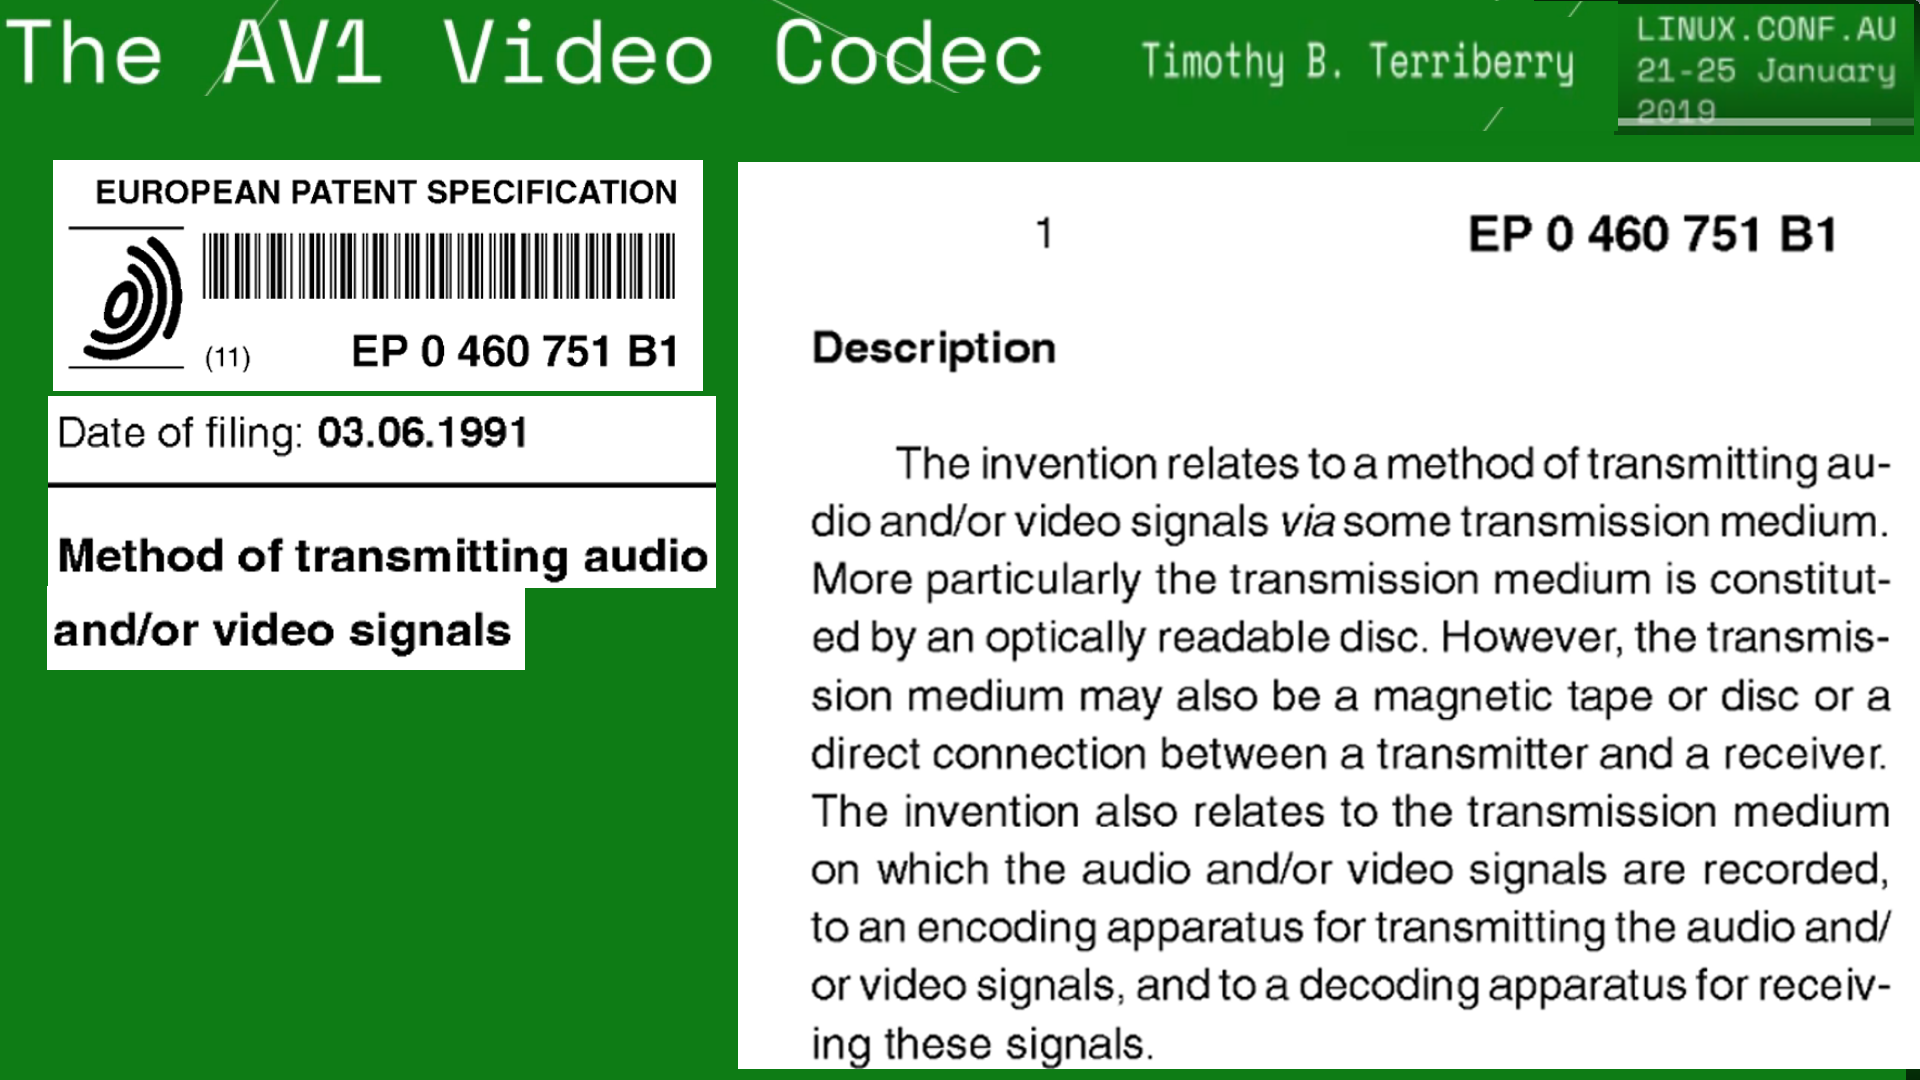
\includegraphics[width=0.9\linewidth]{os01-avw}
\end{figure}
\end{frame}

% XXXXXXXXXXXXXXXXXXXXXXXXXXXXXXXXXXXXXXXXXXXXXXXXXXXXXXXXXXXXXXXXXXXXXXXXXX
\begin{frame}
\frametitle{The Codec Mess}
\begin{figure}
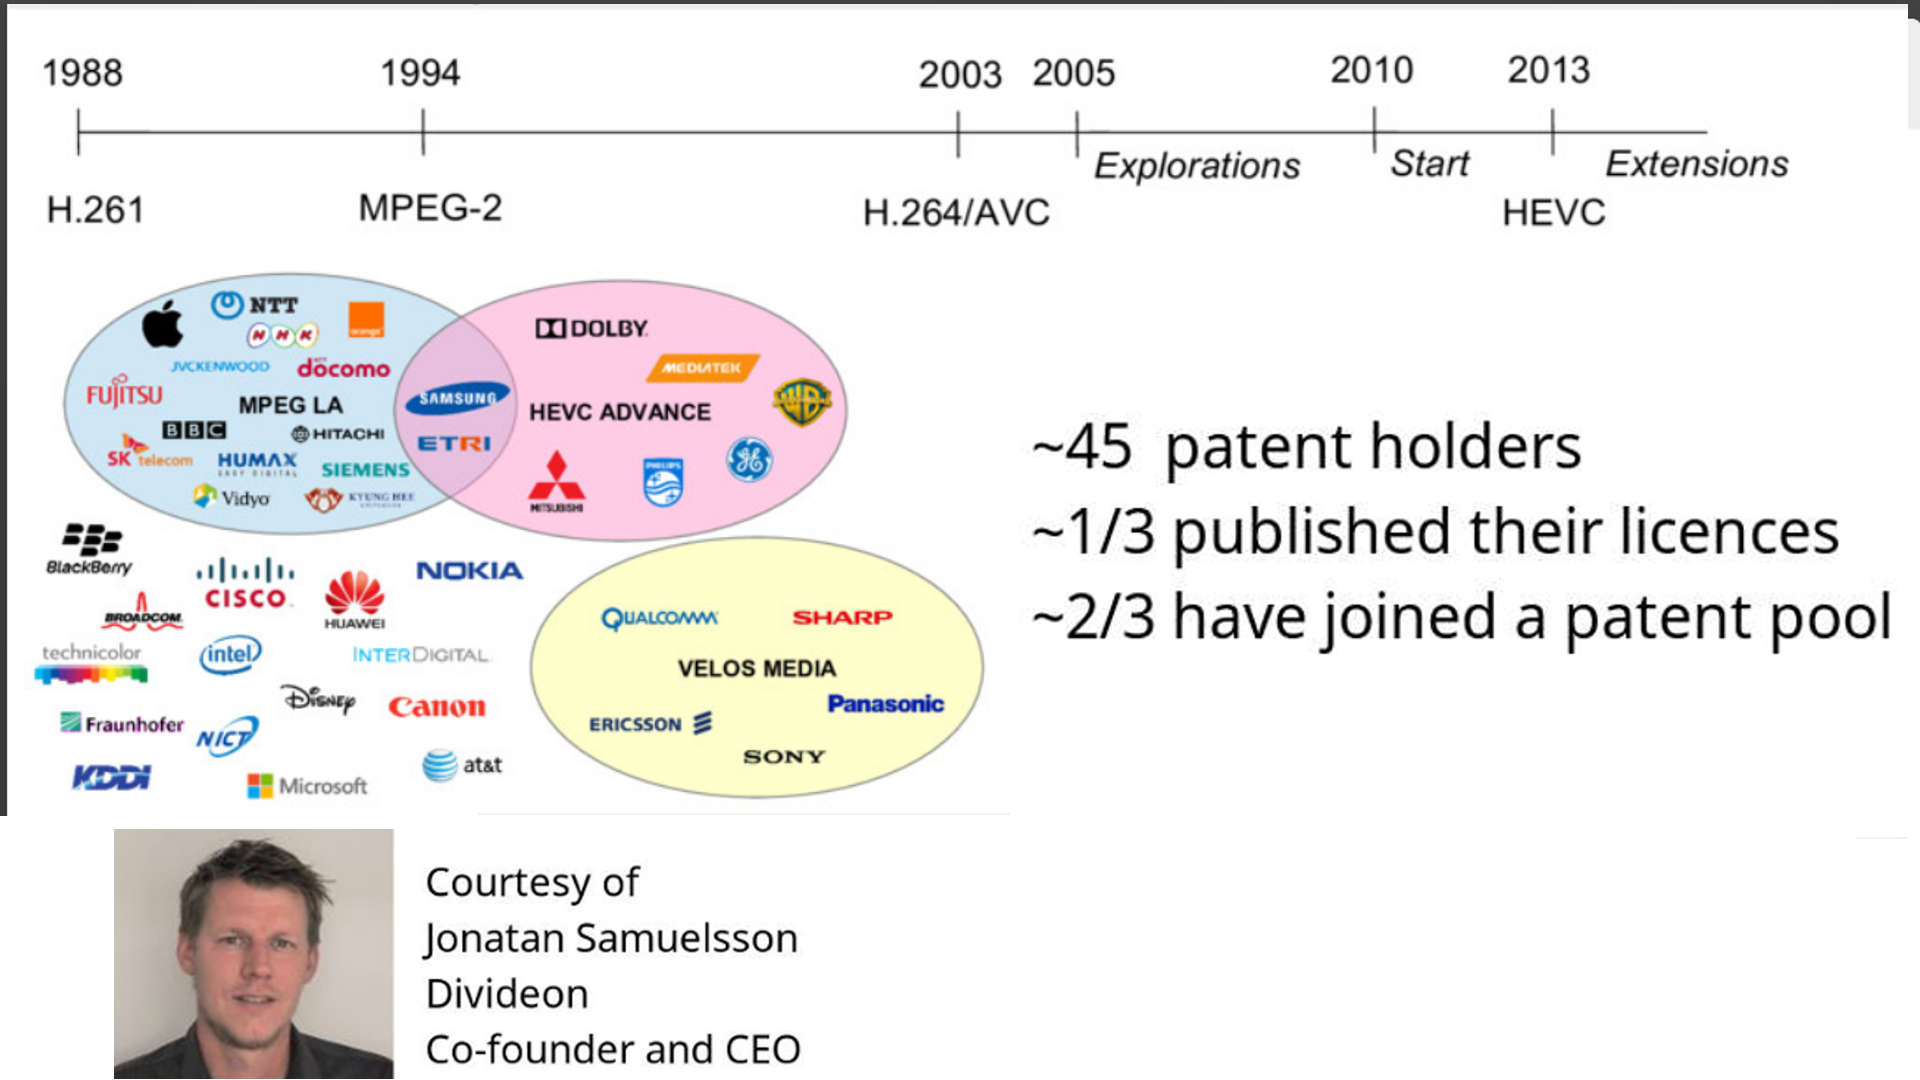
\includegraphics[width=0.99\linewidth]{os01-avx}
\end{figure}
\end{frame}

% XXXXXXXXXXXXXXXXXXXXXXXXXXXXXXXXXXXXXXXXXXXXXXXXXXXXXXXXXXXXXXXXXXXXXXXXXX
\begin{frame}
\frametitle{Alliance for Open Media}
\begin{figure}

\includegraphics[width=0.49\linewidth]{os01-avy}
\end{figure}
{\small Source (per 21-Sep-2020): \url{https://aomedia.org/membership/members/}}
\end{frame}

% XXXXXXXXXXXXXXXXXXXXXXXXXXXXXXXXXXXXXXXXXXXXXXXXXXXXXXXXXXXXXXXXXXXXXXXX
\section{Free Software}
\begin{frame}
\frametitle{Free Software}
\begin{itemize}
\item Free Software Definition (FSF)
\begin{enumerate}
\setcounter{enumi}{-1}
\item The freedom to run the program as you wish, for any purpose (freedom 0).
\item The freedom to study how the program works and change it does your computing 
      as you wish (freedom 1). Access to the source code is a precondition for this.
\item The freedom to redistribute copies so you can help your neighbor (freedom 2).
\item The freedom to distribute copies of your modified versions to others (freedom 3).
      By doing this, you can give the whole community a chance to benefit from your changes.
      Access to the source code is a precondition for this.
\end{enumerate}
\item Free Software vs. Open Source Software.
\item Copyleft Software.
\end{itemize}
\end{frame}

% XXXXXXXXXXXXXXXXXXXXXXXXXXXXXXXXXXXXXXXXXXXXXXXXXXXXXXXXXXXXXXXXXXXXXXXX
\section{Software Licenses}
\begin{frame}
\frametitle{Software Licenses}
\begin{itemize}
\item 3-clause BSD license and 2-clause BSD license (BSD-X-Clause) 
\item Apache License 2.0 (Apache-2.0)
\item Artistic License 2.0 (ArtisticLicense2)
\item Common Development and Distribution License (CDDL-1.0)
\item Eclipse Public License (EPL-1.0)
\item Educational Community License 2.0 (ECL2.0)
\item Expat License (Expat) aka.  MIT license (MIT) 
\item GNU Affero General Public License v3 (AGPL-3.0)
\item GNU All-Permissive License (GNUAllPermissive)
\item GNU General Public License (GPL)
\item GNU Lesser General Public License (LGPL)
\item Microsoft Public License (MS-PL)
\item Mozilla Public License 2.0 (MPL-2.0)
\item ''Public Domain'' (PublicDomain)
\item X11 License (X11License)
\end{itemize}
\end{frame}

% XXXXXXXXXXXXXXXXXXXXXXXXXXXXXXXXXXXXXXXXXXXXXXXXXXXXXXXXXXXXXXXXXXXXXXXX
\section{Virtualization \& Cloud Computing}
\begin{frame}
\frametitle{Virtualization \& Cloud Computing}
\begin{itemize}
\item Virtual Machine
\begin{itemize}
\item Host \& Guest
\item Hypervisor (Virtual Machine Manager)
\begin{itemize}
\item Type 0, 1, 2 Hypervisor
\item ParaVirtualization
\item Programming-environment Virtualization
\item Emulators
\end{itemize}
\item Application Containment (OS-Level)
\begin{itemize}
\item Containers: LXC, Solaris Containers, Docker.
\item Zones: Solaris Containers
\item Virtual Private Servers: OpenVZ
\item Virtual Kernels: DragonFly BSD
\item Jails: FreeBSD Jail/ Chroot Jail
\end{itemize}
\item Kubernetes (K8s): A (open source) system for managing CONTAINERIZED applications.
\end{itemize}
\item Cloud Computing
\begin{itemize}
\item SAAS: Software As A Service.
\item PAAS: Platform As A Service.
\item IAAS: Infrastructure As A Service.
\end{itemize}
\end{itemize}
\end{frame}

% XXXXXXXXXXXXXXXXXXXXXXXXXXXXXXXXXXXXXXXXXXXXXXXXXXXXXXXXXXXXXXXXXXXXXXXXXX
\section{Potpourri}
\begin{frame}
\frametitle{Potpourri}
\begin{itemize}
\item Mobile/Distributed/Client-Server/Peer-to-Peer Computing.
\item Real-Time Computing: Hard Real-Time vs. Soft Real-Time.
\item Operating System Comparison: 
Android, 
*BSD,
GNU/Linux, 
iOS, 
Mac OS, 
Windows.
\item Operating System Services: UI (GUI, CLI); Program Executing; I/O Operations; 
      File Systems Manipulation; Communication; Error Detection; Resource Allocation;
      Accounting; Protection \& Security.
\item System Calls: Process Control; File Management; Device Management; Information
      Maintenance; Communications; Protection.
\item Application Programming Interface (API)
\item Standard C Library.
\item System Programs.
\item Microkernel System Structure.
\item Loadable Kernel Modules.
\item Virtualization and Cloud System.
\end{itemize}
\end{frame}

% XXXXXXXXXXXXXXXXXXXXXXXXXXXXXXXXXXXXXXXXXXXXXXXXXXXXXXXXXXXXXXXXXXXXXXXXXX
\section{Week 01: Assignment \#1: VirtualBox Guest Preparation}
\begin{frame}[fragile]
\frametitle{Week 01: Assignment \#1: VirtualBox Guest Preparation}
\begin{itemize}
\item Visit \url{https://osp4diss.vlsm.org/\#idx00b}.
\item You need a hypervisor (VirtualBox), which can be installed on Windows 10, macOS, or Linux.
\begin{itemize}
\item Downloading and Installing VirtualBox
\url{https://www.virtualbox.org/}
\end{itemize}
\item A Download Manager might help for a less reliable internet.
\begin{itemize}
\item FDM: Free Download Manager (Optional)\\
\url{https://www.freedownloadmanager.org/}
\end{itemize}
\item For Windows 10, you also need to install PUTTY and WINSCP.
\begin{itemize}
\item Visit \url{https://osp4diss.vlsm.org/SSHGuest.html}
\end{itemize}
\item For MacOs, visit: {\scriptsize \url{https://fxdros.github.io/virtualbox-on-macos/}}.
\item Understand how to Import / Export / Delete a Virtual Guest
\begin{itemize}
\item Visit \url{https://osp4diss.vlsm.org/\#idx01}.
\item \href{https://osp4diss.vlsm.org/DebianGuestExportOva.html}{Exporting OVA}
\item \href{https://osp4diss.vlsm.org/DebianGuestImportOva.html}{Importing OVA}
\item \href{https://osp4diss.vlsm.org/ExportImportGuests.html}{Export / Import OVA}
\item \href{https://osp4diss.vlsm.org/DebianGuestDeleteOva.html}{Deleting OVA}
\end{itemize}
\end{itemize}
\end{frame}

% XXXXXXXXXXXXXXXXXXXXXXXXXXXXXXXXXXXXXXXXXXXXXXXXXXXXXXXXXXXXXXXXXXXXXXXXXX
\section{Week 01: Assignment \#2: Importing OVA or Installing ISO?}
\begin{frame}[fragile]
\frametitle{Week 01: Assignment \#2: Importing or Installing?}
\begin{itemize}
\item \textbf{Option 1 or Option 2?}
\begin{itemize}
\item \href{https://osp4diss.vlsm.org/\#idx02a}{Option 1}: 
      You might \textbf{import} a pre-installed OVA file.
\begin{itemize}
\item README: \url{https://bit.ly/3g5lwkX} (452 bytes)
\item Debian 11 OVA for VirtualBox: \url{https://bit.ly/3yQDL4V} (360 MB)
\item See also \url{https://osp4diss.vlsm.org/#idx01}.
\end{itemize}
\item \href{https://osp4diss.vlsm.org/\#idx02b}{Option 2}: 
      You might \textbf{install} a Debian Guest from scratch.
\begin{itemize}
\item Visit \url{https://osp4diss.vlsm.org/\#idx02b}.
      Set an \textbf{EMPTY VIRTUAL GUEST}, General, System, Display, Storage, Audio, Network.
\item \href{https://cdimage.debian.org/debian-cd/current/amd64/iso-cd/}{Download Debian Netinst (ISO)}.
\item \href{https://osp4diss.vlsm.org/InstallDebianNetinst.html}{Installing Debian NetInst (guest)}.
\end{itemize}
\end{itemize}
\item Running a VirtualBox Debian Guest (OVA or ISO)
\begin{itemize}
\item Visit \url{https://osp4diss.vlsm.org/\#idx03}.
\item Try to startup, console login, console log out, and shutdown.
\item Try ssh (or putty) and scp (or winscp).
\item Study some Command Lines, Editor, Regular Expression, and String Processing.
      (See also assignment \#3).
\item Shut down and export your virtual guest (Guest-01a.ova).
\end{itemize}
\end{itemize}

\end{frame}

% XXXXXXXXXXXXXXXXXXXXXXXXXXXXXXXXXXXXXXXXXXXXXXXXXXXXXXXXXXXXXXXXXXXXXXXX
\section{Week 01: Assignment \#3 The ATM Way: GSGS and Read}
\begin{frame}
\frametitle{Week 01: Assignment \#3 The ATM Way: GSGS and Read}

\begin{itemize}
\item Do the \textbf{ATM Way}\footnote{%
Amati, Tiru, Modifikasi. Romi Satria Wahono has been using this term since 2007.}:
\textbf{GSGS}\footnote{Google Sana, Google Sini} and Read!
\begin{itemize}
\item \textbf{REVISIT} \url{https://osp4diss.vlsm.org/Welcome2GNULinux.html}
\begin{itemize}
\item Linux Sucks 2021 \url{https://youtu.be/WtJ9T_IJOPE?t=87}
\item Basic Linux Commands \url{https://youtu.be/CpTfQ-q6MPU} and
{\scriptsize \url{https://linoxide.com/linux-command/essential-linux-basic-commands/}}
\item The Complete Linux Course: Beginner to Power User (7:23 hours) -- \url{https://youtu.be/wBp0Rb-ZJak}
\item Basic vi commands \url{https://youtu.be/ggSyF1SVFr4} and
\url{https://www.cs.colostate.edu/helpdocs/vi.html}.
\item Learn REGEX in 15 minutes \url{https://youtu.be/bgBWp9EIlMM}
\item BASH 
\url{https://tldp.org/LDP/abs/abs-guide.pdf},
\url{https://youtu.be/F-gskSl4pwQ},
\url{https://youtu.be/_n5ZegzieSQ}.
\item SED \url{https://www.gnu.org/software/sed/manual/sed.pdf}
\item GAWK \url{https://www.gnu.org/software/gawk/manual/gawk.pdf}
\item Essential Awk \url{https://youtu.be/9YOZmI-zWok}
\item Linux Man Pages \url{https://youtu.be/uJnrh9hAQR0}
\item The Minix3 Notes: \url{https://rms46.vlsm.org/2/166.pdf}
\end{itemize}
\item \textbf{VISIT} \url{https://osp4diss.vlsm.org/osp-115.html}
\end{itemize}
\end{itemize}
\end{frame}

% XXXXXXXXXXXXXXXXXXXXXXXXXXXXXXXXXXXXXXXXXXXXXXXXXXXXXXXXXXXXXXXXXXXXXXXXXX
\begin{frame}[fragile]
\frametitle{Week 01: Assignment \#3 (1): Learn/Try It}
\begin{itemize}
\item Revisit \url{https://osp4diss.vlsm.org/}
\item Learn basic \textbf{Command-Line Interface} (CLI) commands:
bash,
cat, 
cd, 
cp, 
ls, 
man,
more, 
mv, 
rm, 
touch, 
wc,
vi,
sed,
awk,
git.
\item Learn how to \textbf{turn on} and \textbf{turn off} (shutdown) your Virtual Guest.
\item Learn how to \textbf{login} and \textbf{logout} with \texttt{ssh} or \texttt{putty}.
\item Learn some essential Regular Expression (regex).
\item Learn the concept of a Stream Editor (sed).
\item Learn the concept of a Git, GitHub, and GitHub Pages.
\item Learn the concept of a AWK.
\item Learn the concept of a SCRIPTING.
\item Pick and learn how to use an editor, e.g. (\textbf{vi}).
\end{itemize}
\end{frame}

% XXXXXXXXXXXXXXXXXXXXXXXXXXXXXXXXXXXXXXXXXXXXXXXXXXXXXXXXXXXXXXXXXXXXXXXX
\begin{frame}
\frametitle{Week 01: Assignment \#3 (2): Some Essential Commands}
\begin{tabular}{l l}
\hline
man    & manual. E.g., \texttt{''man man''}                                      \\
passwd & changes passwords.                                                    \\
ls     & list directory contents.  E.g., \texttt{''ls -al''}                     \\
cd     & change the working directory. E.g., \texttt{''cd /tmp''}                \\
cp     & copy file(s). E.g., \texttt{''cp SOURCE DEST''}                         \\
rm     & remove file(s).  E.g., \texttt{''rm AFILE''}                            \\
mv     & move files(s).        E.g., \texttt{''mv FROMFILE TOFILE''}             \\
mkdir  & make directories(s).        E.g., \texttt{''mkdir ADIRECTORY''}         \\
rmdir  & remove directories(s).        E.g., \texttt{''rmdir ADIRECTORY''}       \\
cat    & read file(s)      E.g., \texttt{''cat AFILE''}                          \\
more   & read file(s) per screen      E.g., \texttt{''more AFILE''}              \\
ln     & make a link of a file. E.g., \texttt{''ln -s file sfile''}              \\
grep   & search string ''aword'' inside file.  E.g., \texttt{''grep aword file''} \\
sort   & sort lines of text files. E.g., \texttt{''sort file1.txt''}             \\
top    & display systems task.  E.g., \texttt{''top''}                           \\
find   & E.g., \texttt{''find / -name minix3.iso -print''}. Find from ''/''.     \\
\hline
\end{tabular}
\end{frame}

% XXXXXXXXXXXXXXXXXXXXXXXXXXXXXXXXXXXXXXXXXXXXXXXXXXXXXXXXXXXXXXXXXXXXXXXX
\begin{frame}
\frametitle{Week 01: Assignment \#3 (3): Some Essential Commands}
\begin{tabular}{l l}
\hline
chmod  & E.g. \texttt{''chmod 755 file''}. Change file with access mode 755.    \\
chown  & E.g. \texttt{''chown user file''}. Change owner file to user.          \\
chgrp  & E.g. \texttt{''chgrp other file''}. Change group file to other.        \\
tar    & tape archive file. E.g.                                                \\
       & \texttt{''tar cf /tmp/tfile.tar  dir/''}. Archive ''dir/'' into tfile.tar. \\
       & \texttt{''tar tf /tmp/tfile.tar''}. List tfile.tar.                   \\
       & \texttt{''tar xf /tmp/tfile.tar''}. Extract tfile.tar.                \\
%      E.g. \texttt{''''}  \\
%      E.g. \texttt{''''}  \\
%      E.g. \texttt{''''}  \\
%      E.g. \texttt{''''}  \\
%      E.g. \texttt{''''}  \\
date   & print or set the system date and time. E.g. \texttt{''date +\%Y''}     \\
tee    & read from standard input and write to standard output and files.      \\
       & E.g. \texttt{''ls -al | tee listing.txt''}                             \\
diff   & compare files line by line. E.g. \texttt{''diff file1.txt file2.txt''} \\
wc     & print newline, word, and byte counts for each file.                   \\
       & E.g. \texttt{''wc file.txt''}                                          \\
\hline
\end{tabular}
\end{frame}

% XXXXXXXXXXXXXXXXXXXXXXXXXXXXXXXXXXXXXXXXXXXXXXXXXXXXXXXXXXXXXXXXXXXXXXXX
\section{Week 01: Assignment \#3 (4): The ''vi'' editor}
\begin{frame}
\frametitle{Week 01: Assignment \#3 (4): The ''vi'' editor}
\begin{itemize}
\item VI Basics
\scalebox{0.75}{%
\begin{tabular}{ll||ll}
  & Basics                               &             & More Commands \\
\hline
i         & insert mode                  & d\^{}       & delete from \^{} (beginning) to the cursor   \\
a         & append mode                  & d\${}       & delete from the cursor to \${} (end)         \\
$<$ESC$>$ & escape mode                  & dd          & delete the whole line                        \\
q!        & quit                         & 5dd         & delete 5 lines                               \\
wq!       & write and quit               & yy          & yank (copy) the line                         \\
ZZ        & write and quit               & p           & put (paste) the line                         \\
h j k l   & move [left, down, up, right] & J           & joint current and next line                  \\
r         & replace a character          & :r file.txt & read (insert) file.txt                       \\
d         & delete  a character          & :w! file.txt & write into file.txt \\
u         & undo                         & :1,8 w! file.txt & write line 1 to 8 into file.txt \\
\hline
\end{tabular}
}
\begin{itemize}
\item Basic vi Commands \url{https://www.cs.colostate.edu/helpdocs/vi.html}
\item Vim Basics in 8 Minutes \url{https://youtu.be/ggSyF1SVFr4}
\end{itemize}
\end{itemize}

\end{frame}

% XXXXXXXXXXXXXXXXXXXXXXXXXXXXXXXXXXXXXXXXXXXXXXXXXXXXXXXXXXXXXXXXXXXXXXXX
\section{Week 01: Assignment \#4: Dress Up Your Virtual Guest}
\begin{frame}[fragile]
\frametitle{Week 01: Assignment \#4: Dress Up Your Virtual Guest}
\begin{itemize}
\item See \url{https://osp4diss.vlsm.org/\#idx04}.
\item Rename Guest as \texttt{Guest-01b.ova}
\item \href{https://osp4diss.vlsm.org/osp-116.html}{PASTE: passing ''NEW LINE'' or not?}
\item \href{https://osp4diss.vlsm.org/osp-102.html}{Update Your Debian Guest}
\item \href{https://osp4diss.vlsm.org/osp-103.html}{Adding Debian Packages}
\item Your Virtual Guest Account should be $==$ Your GitHub Account.
E.g., ''\texttt{cbkadal}''. See \href{https://osp4diss.vlsm.org/osp-104.html}{Adding User Name}
\item Your Virtual Guest Account should be $==$ Your Virtual Hostname.
E.g., ''\texttt{cbkadal}''. See \href{https://osp4diss.vlsm.org/osp-105.html}{Rename a Hostname}
\item \href{https://osp4diss.vlsm.org/osp-106.html}{Create/Edit ''.bash\_profile''}
\item \href{https://osp4diss.vlsm.org/osp-107.html}{Create/Edit ''.vimrc''}
\item \href{https://osp4diss.vlsm.org/osp-108.html}{Create/Edit ''.bash\_aliases''}
\item \href{https://osp4diss.vlsm.org/osp-109.html}{SUPERUSER}
\item Export Guest as \texttt{Guest-01b.ova}
\end{itemize}
\end{frame}


% XXXXXXXXXXXXXXXXXXXXXXXXXXXXXXXXXXXXXXXXXXXXXXXXXXXXXXXXXXXXXXXXXXXXXXXX
\section{Week 01: Assignment \#5: SSH Keys and Git Cloning}
\begin{frame}[fragile]
\frametitle{Week 01: Assignment \#5: SSH Keys and Git Cloning}
\begin{itemize}
\item See \url{https://osp4diss.vlsm.org/\#idx05}.
\item Rename Guest as \texttt{Guest-01c.ova}
\item \href{https://osp4diss.vlsm.org/osp-110.html}{SSH: Generating public/private RSA key pair}
\item \href{https://osp4diss.vlsm.org/osp-111.html}{SSH: Put a Public Key at GitHub.com (e.g. cbkadal)}
\item \href{https://osp4diss.vlsm.org/osp-112.html}{GIT: .gitconfig}
\item \href{https://osp4diss.vlsm.org/osp-113.html}{GIT: cloning from GitHub.com}
\end{itemize}
\end{frame}


% XXXXXXXXXXXXXXXXXXXXXXXXXXXXXXXXXXXXXXXXXXXXXXXXXXXXXXXXXXXXXXXXXXXXXXXX
\section{Week 01: Assignment \#6: Dress Up Your GitHub Page}
\begin{frame}[fragile]
\frametitle{Week 01: Assignment \#6: Dress Up Your GitHub Page}
\begin{itemize}
\item GSGS about the Markdown (MD) markup language.
\begin{itemize}
\item See {\scriptsize \url{https://github.com/adam-p/markdown-here/wiki/Markdown-Cheatsheet}.}
\item See \url{https://doit.vlsm.org/003.html}
\item See \url{https://template.vlsm.org/}. 
      You may want to download \url{https://template.vlsm.org/template.zip}
\end{itemize}
\item (If not yet) Create MD file ''index.md'' with empty front-matter.
\begin{itemize}
\item Add links to ''TXT/mylog.txt'', ''GitHub'' and ''/LINKS/'' (see below).
\end{itemize}
\item Create an MD file ''links.md'' with front-matter {\scriptsize ''\texttt{permalink: /LINKS/}.''}
\begin{itemize}
\item Fill the page with links that (you think) are helpful for this Operating Systems course.
      Add to each link two or more sentences:
\begin{itemize}
\item what the link is about
\item why you think the link is interesting.
\end{itemize}
\item From next week, the links will be \textbf{peer-reviewed}.
\item For example, see \texttt{cbkadal}'s:
\begin{itemize}
\item GitHub Page at \url{https://cbkadal.github.io/os212/LINKS/}.
\item {\scriptsize \url{https://raw.githubusercontent.com/cbkadal/os212/master/links.md}}.
\end{itemize}
\end{itemize}
\item Your links may appear next semester in \url{https://osp4diss.vlsm.org/osp-115.html}.
\end{itemize}
\end{frame}

% XXXXXXXXXXXXXXXXXXXXXXXXXXXXXXXXXXXXXXXXXXXXXXXXXXXXXXXXXXXXXXXXXXXXXXXX
\section{Week 01: Assignment \#7: Update mylog.txt}
\begin{frame}[fragile]
\frametitle{Week 01: Assignment \#7: Update mylog.txt}
\begin{itemize}
\item \href{https://osp4diss.vlsm.org/osp-114.html}{mylog: Updating add commit push}
\begin{itemize}
\item With your favorite editor (perhaps ''vi''?), update file mylog.txt.
\end{itemize}
\item See \url{https://osp4diss.vlsm.org/ETC/logCodes.txt} for the Code list.
\item \textbf{PUSH BACK} your repo into GitHub.com!
\item Always remember the \textbf{4 Git Mantras}:
\begin{lstlisting}[basicstyle=\ttfamily\footnotesize]
git pull
git add -A
git commit
git push
\end{lstlisting}
\item Export Guest as \texttt{Guest-01c.ova}
\end{itemize}
\end{frame}

% XXXXXXXXXXXXXXXXXXXXXXXXXXXXXXXXXXXXXXXXXXXXXXXXXXXXXXXXXXXXXXXXXXXXXXXX
\section{Week 01: Assignment \#8: More awk, bash, regex, sed}
\begin{frame}[fragile]
\frametitle{Week 01: Assignment \#8 (1): More awk, bash, regex, sed}
\begin{itemize}
\item awk
\begin{itemize}
\item \texttt{awk '\{print ''Hello awk!''\}' file.txt} --- print ''Hello awk!'' for every file.txt line.
\item \texttt{awk '\{print \$0\}' file.txt} --- print every file.txt line.
\item \texttt{awk '\{print \$1\}' file.txt} --- print first field of every file.txt line.
\item \texttt{awk '\{print \$2\}' file.txt} --- print second field of every file.txt line.
\end{itemize}
\item regex
\begin{itemize}
\item to search patterns
\item BRE (Basic Regular Expression) vs ERE (Extended Regular Expression)
\item Flavors: Grep, Java, JavaScript, PHP, POSIX, Python, sed, XML, \ldots
\end{itemize}
\end{itemize}
\end{frame}

% ZCZC
% XXXXXXXXXXXXXXXXXXXXXXXXXXXXXXXXXXXXXXXXXXXXXXXXXXXXXXXXXXXXXXXXXXXXXXXX
\begin{frame}[fragile]
\frametitle{Week 01: Assignment \#8 (2): bash, regex, sed, and awk}
\begin{itemize}
\item $\ll$\texttt{\^{}\${}}$\gg$ --- matches a beginning-of-line + end-of-line (empty line).
\begin{itemize}
\item $\ll$\texttt{\^{}}$\gg$ --- matches a beginning-of-line (meaningless).
\item $\ll$\texttt{\^{}hello\${}}$\gg$ --- matches just ''hello'' in a line.
\end{itemize}
\item $\ll${\tiny{}\textbullet}$\gg$ --- matches any character.
\begin{itemize}
\item $\ll$\texttt{hell.}$\gg$ --- matches ''hellA'', ''hella'', ''hellB'', ''hellb'', \ldots
\end{itemize}
\item $\ll$\texttt{[AB]}$\gg$ --- matches ''A'' or ''B'' only.
\begin{itemize}
\item $\ll$\texttt{[0-3]}$\gg$ --- matches ''0'', ''1'', ''2'', or ''3'' only.
\item $\ll$\texttt{[\^{}4-9]}$\gg$ --- not match ''4'', ''5'', ''6'', ''7'', ''8'', or ''9''.
\end{itemize}
\item $\ll$\texttt{?}$\gg$ --- matches preceding zero or one time.
\begin{itemize}
\item $\ll$\texttt{a?b}$\gg$ --- matches ''b'' or ''ab'' only.
\end{itemize}
\item $\ll$\texttt{*}$\gg$ --- matches preceding zero or more times.
\begin{itemize}
\item $\ll$\texttt{a*b}$\gg$ --- matches ''b'' or ''ab'' or ''aab'' or \ldots
\item $\ll$\texttt{A.*Z}$\gg$ --- matches ''AZ'' or ''AaZ'' or ''AabZ'' or \ldots
\end{itemize}
\item $\ll$\texttt{+}$\gg$ --- matches preceding one or more times.
\begin{itemize}
\item $\ll$\texttt{a+b}$\gg$ --- matches ''ab'', ''aab'', ''aaab'', \ldots
\end{itemize}
\item $\ll$\texttt{\{\}}$\gg$ --- matches numbers in \{\}.
\begin{itemize}
\item $\ll$\texttt{a\{2\}}$\gg$ --- matches ''aa''.
\item $\ll$\texttt{a\{2,5\}}$\gg$ --- matches ''aa'', ''aaa'', ''aaaa'', and ''aaaaa''.
\item $\ll$\texttt{a\{2,\}}$\gg$ --- matches ''aa'', ''aaa'', ''aaaa'', ''aaaaa'', \ldots
\end{itemize}
\end{itemize}
\end{frame}

% XXXXXXXXXXXXXXXXXXXXXXXXXXXXXXXXXXXXXXXXXXXXXXXXXXXXXXXXXXXXXXXXXXXXXXXX
\begin{frame}[fragile]
\frametitle{Week 01: Assignment \#8 (3): bash, regex, sed, and awk}
\begin{itemize}
\item $\ll$\texttt{\textbackslash}$\gg$ --- escape character.
\item $\ll$\texttt{\textbackslash}0$\gg$ --- NULL.
\item $\ll$\texttt{\textbackslash}b$\gg$ --- word boundary.
\item $\ll$\texttt{\textbackslash}B$\gg$ --- non-word boundary.
\item $\ll$\texttt{\textbackslash}d$\gg$ --- any digit. E.g. $\ll$\texttt{\textbackslash}d\{1,3\}$\gg$
      = \texttt{0 -- 999}.
\item $\ll$\texttt{\textbackslash}D$\gg$ --- any non-digit.
\item $\ll$\texttt{\textbackslash}n$\gg$ --- new line.
\item $\ll$\texttt{\textbackslash}t$\gg$ --- tab.
\item $\ll$\texttt{\textbackslash}s$\gg$ --- white space character.
\item $\ll$\texttt{\textbackslash}S$\gg$ --- non white space character.
\end{itemize}
\end{frame}

% XXXXXXXXXXXXXXXXXXXXXXXXXXXXXXXXXXXXXXXXXXXXXXXXXXXXXXXXXXXXXXXXXXXXXXXX
\begin{frame}[fragile]
\frametitle{Week 01: Assignment \#8 (4): bash, regex, sed, and awk}
\begin{itemize}
\item $\ll$\texttt{(\ldots)}$\gg$ --- group.
\begin{itemize}
\item $\ll$\texttt{(?:\ldots)}$\gg$ --- passive group.
\item $\ll$\texttt{(regex)$\mid$(regex)}$\gg$ --- matches left regex or right regex.
\item $\ll$\texttt{(a\textbar{}b}$\gg$ --- matches either a or b.
\item $\ll$\texttt{\^{}(From\textbar{}To):}$\gg$ --- matches either $\ll$\texttt{\^{}From:}$\gg$ or
      $\ll$\texttt{\^{}To:}$\gg$.
\end{itemize}
\item $\ll$\texttt{[0-9]\{10\}}$\gg$ --- 10 digits.
\item $\ll$\texttt{0[0-9]|1[0-9]|2[0-3]):[0-5][0-9]}$\gg$ --- 00:00--23:59.
\item $\ll$\texttt{([0-9]|0[0-9]|1[0-9]|2[0-3]):[0-5][0-9]}$\gg$ --- (0)0:00--23:59.
\end{itemize}
\end{frame}


% XXXXXXXXXXXXXXXXXXXXXXXXXXXXXXXXXXXXXXXXXXXXXXXXXXXXXXXXXXXXXXXXXXXXXXXX
\begin{frame}[fragile]
\frametitle{Week 01: Assignment \#8 (5): bash, regex, sed, and awk}
\begin{itemize}
\item $\ll$\texttt{[:alnum:]}$\gg$ --- alpha-numerics.
\item $\ll$\texttt{[:alpha:]}$\gg$ --- alphabets
\item $\ll$\texttt{[:blank:]}$\gg$ --- spaces and tabs.
\item $\ll$\texttt{[:digit:]}$\gg$ --- digits.
\item $\ll$\texttt{[:lower:]}$\gg$ --- lower case.
\item $\ll$\texttt{[:space:]}$\gg$ --- spaces.
\item $\ll$\texttt{[:upper:]}$\gg$ --- upper case.
\item $\ll$\texttt{[:xdigit:]}$\gg$ --- hexadecimal digits.
\item $\ll$\texttt{[:punct:]}$\gg$ --- punctuation.
\item $\ll$\texttt{[:cntrl:]}$\gg$ --- control characters.
\item $\ll$\texttt{[:graph:]}$\gg$ --- printed characters.
\item $\ll$\texttt{[:print:]}$\gg$ --- printed and spaces.
\item $\ll$\texttt{[:word:]}$\gg$ --- alpha-numerics and underscore.
\end{itemize}
\end{frame}

% XXXXXXXXXXXXXXXXXXXXXXXXXXXXXXXXXXXXXXXXXXXXXXXXXXXXXXXXXXXXXXXXXXXXXXXXXX
\begin{frame}[fragile]
\frametitle{Week 01: Assignment \#8 (6): bash, regex, sed, and awk}

\begin{verbatim}
\b(?:(?:25[0-5]|2[0-4]\d|[01]?\d\d?)\.){3}
(?:25[0-5]|2[0-4]\d|[01]?\d\d?)\b
\end{verbatim}

\begin{figure}
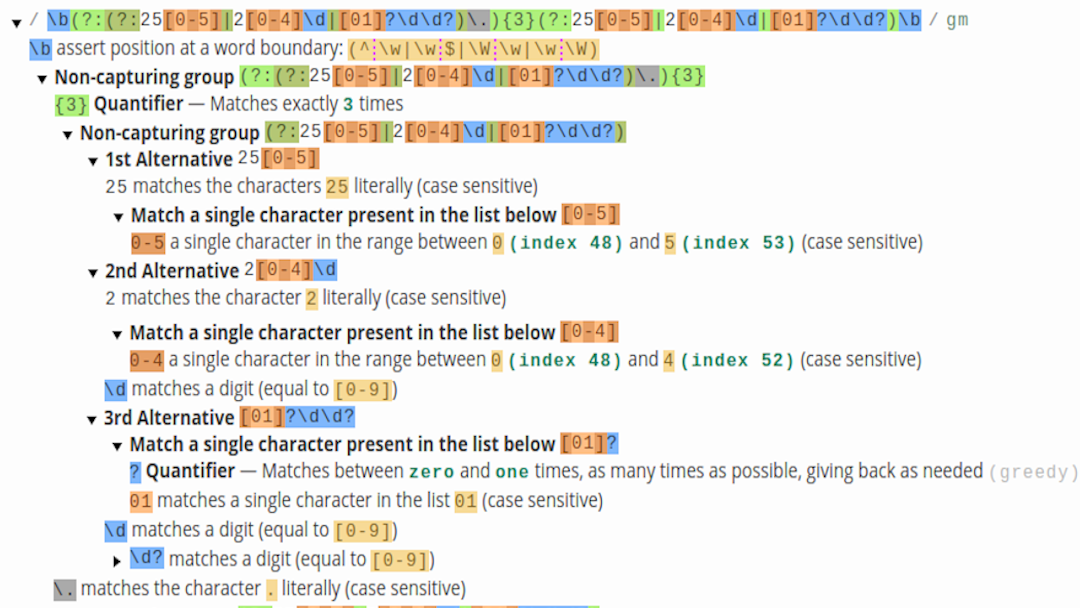
\includegraphics[width=0.96\linewidth]{os-regex1}
\end{figure}
\end{frame}

% XXXXXXXXXXXXXXXXXXXXXXXXXXXXXXXXXXXXXXXXXXXXXXXXXXXXXXXXXXXXXXXXXXXXXXXXXX
\begin{frame}[fragile]
\frametitle{Week 01: Assignment \#8 (8): bash, regex, sed, and awk}

\begin{verbatim}
\b(?:(?:25[0-5]|2[0-4]\d|[01]?\d\d?)\.){3}
(?:25[0-5]|2[0-4]\d|[01]?\d\d?)\b
\end{verbatim}

\begin{figure}
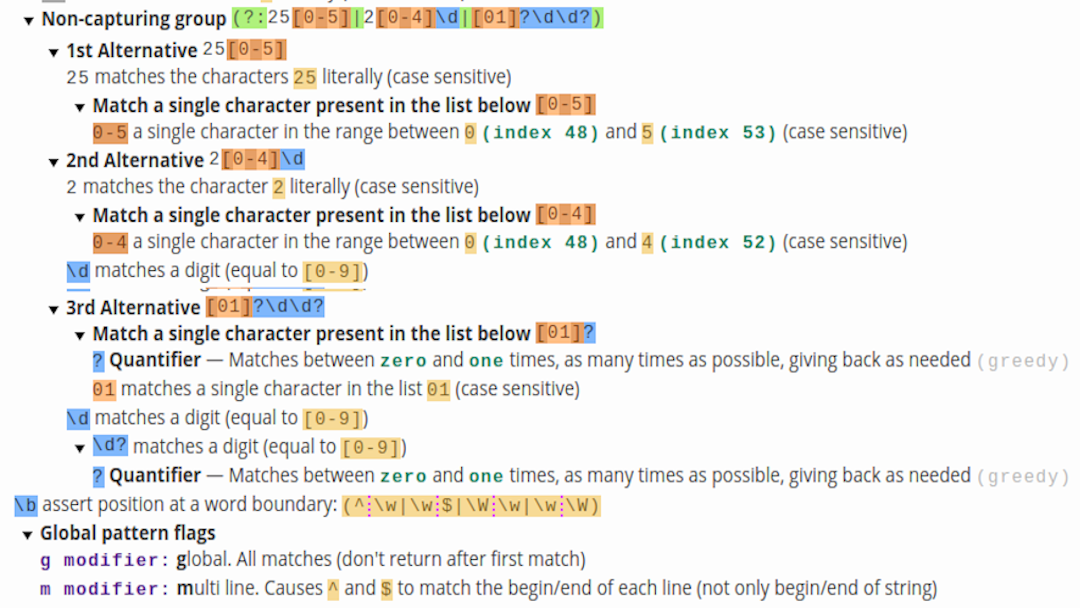
\includegraphics[width=0.96\linewidth]{os-regex2}
\end{figure}
\end{frame}

% XXXXXXXXXXXXXXXXXXXXXXXXXXXXXXXXXXXXXXXXXXXXXXXXXXXXXXXXXXX
\begin{frame}[fragile]
\frametitle{Week 01: Assignment \#8 (9): bash, regex, sed, and awk}
\begin{lstlisting}[basicstyle=\ttfamily\tiny]

# file.txt

1. This is no. 1.
2. This is no. 22.
3. This is no. 333.  
4. This is no. 4 4 4 4.
5. This is Joko.
6. This is Joko Joko.
7. This is joko.
8. This is Bowo.
9. This is bowo.
sed    'G'    ZA-thisfile1.txt
sed    'G;G'  ZA-thisfile1.txt
sed -n '4,6p' ZA-thisfile1.txt
sed -n '4,6p' ZA-thisfile1.txt > ZA-thisfile2.txt
sed -n '/[0-9]\{2\}/p' ZA-thisfile1.txt
sed    '4,6d' ZA-thisfile1.txt
sed    '$d' ZA-thisfile1.txt
sed    '5,/HABATS/d'   ZA-thisfile1.txt
sed    's/Joko/Bowo/'   ZA-thisfile1.txt
sed    's/Joko/Bowo/2' ZA-thisfile1.txt
sed    's/Joko/Bowo/g' ZA-thisfile1.txt
sed    's/Bowo\|bowo/Joko/g' ZA-thisfile1.txt
awk    '{print "Hello awk!"}' ZA-thisfile1.txt
awk    '{print $0}' ZA-thisfile1.txt
awk    '{print $1}' ZA-thisfile1.txt
awk    '{print $2}' ZA-thisfile1.txt
HABATS: This is the last line, dude!

\end{lstlisting}
\end{frame}


% NNNN
% XXXXXXXXXXXXXXXXXXXXXXXXXXXXXXXXXXXXXXXXXXXXXXXXXXXXXXXXXXXXXXXXXXXXXXXX
\begin{frame}[fragile]
\frametitle{Week 01: Assignment \#8 (10): bash, regex, sed, and awk}
\begin{itemize}
\item \texttt{sed 'G'    file.txt} --- double space.
\item \texttt{sed 'G;G'  file.txt} --- triple space.
\item \texttt{sed -n '4,6p'  file.txt} --- show only line 4 to 6.
\item \texttt{sed -n '4,6p'  file.txt > newfile.txt} --- write line 4 to 6 to newfile.txt.
\item \texttt{sed '/[0-9]\textbackslash\{2\textbackslash\}/p' file.txt} --- show only lines with two digits. 
\item \texttt{sed '4,6d'     file.txt} --- show all except line 4 to 6.
\item \texttt{sed '\$d'      file.txt} --- show all except last line.
\item \texttt{sed '5,/HABATS/d'} --- show all except from line 5 to a line with HABATS.
\item \texttt{sed 's/Joko/Bowo/'  file.txt} --- replace Joko with Bowo.
\item \texttt{sed 's/Joko/Bowo/2' file.txt} --- replace the second Joko with Bowo.
\item \texttt{sed 's/Joko/Bowo/g' file.txt} --- replace every Joko with Bowo.
\item \texttt{sed 's/Bowo\textbackslash{}|bowo/Joko/g' file.txt} -- replace every Bowo or bowo with Joko.
\end{itemize}
\end{frame}

% XXXXXXXXXXXXXXXXXXXXXXXXXXXXXXXXXXXXXXXXXXXXXXXXXXXXXXXXXXXXXXXXXXXXXXXX
\section{Week 01: Assignment \#9: OSC 10}
\begin{frame}[fragile]
\frametitle{Week 01: Assignment \#9: OSC 10}
\begin{itemize}
\item Read: (OSC10 chapter 1 + chapter 2 + chapter 18)
\end{itemize}
\end{frame}

% XXXXXXXXXXXXXXXXXXXXXXXXXXXXXXXXXXXXXXXXXXXXXXXXXXXXXXXXXXXXXXXXXXXXXXXXXX

% %%%%%%%%%%%%%%%%%%%%%%%%%%%%%%%%%%%%%%%%%%%%%%%%%%%%%%%%%%%%%%%%%%%%%%%
% Beamer Presentation - LaTeX - Template Version 1.0 (10/11/12)
% This template has been downloaded from: http://www.LaTeXTemplates.com
% License: % CC BY-NC-SA 3.0 (http://creativecommons.org/)
% Modified by Rahmat M. Samik-Ibrahim

% REV341 Sun 05 Sep 2021 23:30:00 WIB
% REV339 Sat 04 Sep 2021 12:50:36 WIB
% REV309 Mon 05 Jul 2021 15:32:10 WIB
% REV285 Sat 13 Mar 2021 06:25:04 WIB
% REV276 Mon 08 Mar 2021 16:50:53 WIB
% STARTX Sun Sep 13 08:49:47 WIB 2020
% %%%%%%%%%%%%%%%%%%%%%%%%%%%%%%%%%%%%%%%%%%%%%%%%%%%%%%%%%%%%%%%%%%%%%%%%

% XXXXXXXXXXXXXXXXXXXXXXXXXXXXXXXXXXXXXXXXXXXXXXXXXXXXXXXXXXXXXXXXXXXXXXXXXX
\section{Week 01: Check List}
\begin{frame}
\frametitle{Week 01: Check List (Deadline: 12 Sep 2021).}
\begin{itemize}
\item [$\square$] This page is \url{https://os.vlsm.org/Slides/check01.pdf}.
\item [$\square$] \textbf{Starting Point:} \url{https://os.vlsm.org/}
\item [$\square$] Week 01: Assignment (more details in \href{https://os.vlsm.org/Slides/os01.pdf}{\textbf{os01.pdf}}).
\begin{enumerate}
\item VirtualBox Guest Preparation
\item Importing (OVA) or Installing (ISO)?
\item Do the ATM way: GSGS and Read!
\item Dress Up Your Virtual Guest
\item SSH Keys and Git Mantras
\item Dress Up Your GitHub Page (index.md and links.md)
\item Update mylog.txt
\item More awk, bash, regex, sed
\item Read: (OSC10 chapter 1 + chapter 2 + chapter 18)
\end{enumerate}
\end{itemize}
\end{frame}



% 12 XXXXXXXXXXXXXXXXXXXXXXXXXXXXXXXXXXXXXXXXXXXXXXXXXXXXXXXXXXXXXXXXXXXXXXX
% XXXXXXXXXXXXXXXXXXXXXXXXXXXXXXXXXXXXXXXXXXXXXXXXXXXXXXXXXXXXXXXXXXXXXXXXXX
\section{The End}
\begin{frame}
\frametitle{The End}
\begin{itemize}
\item[$\square$] This is the end of the presentation.
\item[$\boxtimes$] This is the end of the presentation.
\item This is the end of the presentation.
\end{itemize}
\end{frame}

% XXXXXXXXXXXXXXXXXXXXXXXXXXXXXXXXXXXXXXXXXXXXXXXXXXXXXXXXXXXXXXXXXXXXXXXXXX
\end{document}

